%!TEX ROOT=formularioFisica.tex

\section{Termodinamica}\label{sec:termodinamica}
La termodinamica si occupa di studiare come un sistema si modifica e interagisce con gli altri
alla variazione di \emph{temperatura}, \emph{pressione} e \emph{volume}.\\
Si tenga conto che $t$ rappresenta la temperatura in \textcelsius\ e $T$ in $K$. Si ricordi che
\begin{equation*}
  C = K + 273.15
\end{equation*}
Per gli esercizi si vada a pagina~\pageref{ex:termodinamica}.

\subsection{Dilatazione}
I solidi, a parte rarissime eccezioni, quando riscaldati si dilatano, quando raffreddati si
contraggono.\\
Ci sono 3 tipi di dilatazione: lineare (che studia la dilatazione su una dimensione), superficiale 
(due dimensioni) e volumetrica (tre dimensioni).

\subsubsection{Lineare}
\begin{equation*}
  l = l_0\left(1+\lambda\Delta t\right)
\end{equation*}
\begin{equation*}
  \Delta l = l_0\lambda\Delta t
\end{equation*}
$\lambda$: coefficiente di dilatazione lineare\\
$l_0$: lunghezza iniziale\\
$\Delta l$: variazione di lunghezza

\subsubsection{Superficiale}
\begin{equation*}
  S = S_0\left(1+\beta\Delta t\right)
\end{equation*}
\begin{equation*}
  \Delta S = S_0\beta\Delta t
\end{equation*}
$\beta$: $2\lambda$, coefficiente di dilatazione superficiale\\
$S_0$: superficie iniziale\\
$\Delta S$: variazione di superficie

\subsubsection{Volumetrica}
\begin{equation*}
  V = V_0\left(1+\alpha\Delta t\right)
\end{equation*}
\begin{equation*}
  \Delta V = V_0\alpha\Delta t
\end{equation*}
$\alpha$: $3\lambda$, coefficiente di dilatazione volumetrica\\
$V_0$: volume iniziale\\
$\Delta V$: variazione di volume

\subsection{Equazione di stato dei gas perfetti}
Questa è l'equazione più generale dei gas.
\begin{equation*}
  \frac{p_1V_1}{T_1} = \frac{p_2V_2}{T_2}
\end{equation*}
Questa proprietà è indispensabile in alcuni esercizi in quanto mette in relazione due situazioni e
permette di trovare tutte le caratteristiche.

\subsection{Prima legge di Gay-Lussac}
Quando $p = \text{costante}$, vi è una trasformazione isobara.
\begin{equation*}
  V = \frac{V_0}{T_0}T
\end{equation*}

\subsection{Seconda legge di Gay-Lussac}
Quando $V = \text{costante}$, vi è una trasformazione isocora.
\begin{equation*}
  p = \frac{p_0}{T_0}T
\end{equation*}

\subsection{Legge di Boyle-Mariotte}
Quando $T = \text{costante}$, vi è una trasformazione isoterma.
\begin{equation*}
  pV = \text{costante}
\end{equation*}

\subsection{Moli e gas perfetti}

\subsubsection{Equazione di stato dei gas perfetti}
Attraverso lo studio sperimentale, Amedeo Avogadro notò una relazione tra pressione, temperatura
e volume assieme al numero di moli che riassunse in
\begin{equation*}
  pV = nRT
\end{equation*}
\hyperref[tab:R]{$R$}: $0.0821\,\text{l}\cdot\text{atm/n}\cdot\text{K}$,
$8.31\,\text{J/K}\cdot\text{mol}$\\
$n$: numero di moli\\ [\baselineskip]
$1\,\text{mol}$ a $273\,\text{K}$, a pressione ambiente di ogni gas occupa $22.4\,\text{L}$.

\subsubsection{Numero di molecole}
\begin{equation*}
  N = n \cdot N_A
\end{equation*}
$n$: numero di moli\\
\hyperref[tab:Na]{$N_A$}: $6.02\,\cdot10^{23}$

\subsubsection{Massa molare}
\begin{equation*}
  M = \frac{m}{n}
\end{equation*}
$m$: massa\\
$n$: numero di moli

\subsection{Teoria Cinetico-Molecolare}
La teoria cinetico-molecolare descrive i movimenti delle molecole all'interno di un gas.\\
Si trova molto spesso in questa sottosezione e nelle successive $l$, ovvero il grado di libertà 
del corpo, ovvero la libertà di movimento di una molecola\\
\begin{center}
  \begin{tabular}{c c}
    $\boldsymbol{l}$ & \textbf{Tipo di Gas}\\ \hline
    $3$ & Monoatomico \\ \hline
    $5$ & Biatomico\\
  \end{tabular}
\end{center}
Queste formule mettono in relazione il macroscopico (forza e pressione) e microscopico (forza e 
pressione di un dato numero di molecole) in un contenitore di gas perfetto.

\begin{center}
  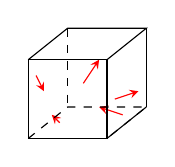
\begin{tikzpicture}		
    \draw[red, -stealth] (0.4,0.2) -- ++(-0.1,0.1);
    \draw[red, -stealth] (0.1,0.8) -- ++(0.1,-0.2);
    \draw[red, -stealth] (1.1,0.5) -- ++(0.3,0.1);
    \draw[red, -stealth] (0.7,0.7) -- ++(0.2,0.3);
    \draw[red, -stealth] (1.2,0.3) -- ++(-0.3,0.1);

    \draw (0,0) -- ++(1,0) -- ++(0,1) -- ++(-1,0) -- cycle;
    \draw[dashed] (0,0) -- ++(0.5,0.4) -- ++(1,0) -- ++(-0.5,-0.4);
    \draw (0,1) -- ++(0.5,0.4) -- ++(1,0) -- ++(-0.5,-0.4);
    \draw[dashed] (0.5,1.4) -- ++(0,-1);
    \draw (1.5,1.4) -- ++(0,-1);
    \draw (1,0) -- ++(0.5,0.4);
  \end{tikzpicture}
\end{center}

\subsubsection{Forza su una parete}
\begin{equation*}
  F_{\text{parete}} = \frac{N}{3}\frac{m}{l}\left\langle v\right\rangle^2
\end{equation*}
$N$: numero di molecole\\
$\left\langle v\right\rangle$: velocità media

\subsubsection{Pressione su una parete}
La pressione misurata è dovuta dalla spinta delle molecole
\begin{equation*}
  p_{\text{parete}}=\frac{N}{3}\frac{m}{V}\left\langle v\right\rangle^2 = \frac{2}{3}\frac{NE_c}{V}
\end{equation*}
$N$: numero di molecole\\
$V$: volume\\
$\left\langle v\right\rangle$: velocità media\\
$E_c$: energia cinetica\\

\subsubsection{Energia cinetica di una molecola}
\begin{equation*}
  E_c = \frac{l}{2}\frac{R}{N}T = \frac{l}{2}k_BT
\end{equation*}
\hyperref[tab:R]{$R$}: $0.0821\,\text{l}\cdot\text{atm/n}\cdot\text{K}$
$8.31\,\text{J/K}\cdot\text{mol}$\\
\hyperref[tab:kB]{$k_B$}: $1.318\cdot10^{-23}\,\text{J/K}$\\
$T$: temperatura in Kelvin\\[\baselineskip]

Si può quindi capire che più un corpo è caldo, maggiore è la quantità di energia cinetica che possiede,
ovvero possiede molecole ad una velocità media sempre più alta.

\subsubsection{Energia interna}
In gas perfetti, l'energia potenziale tra le molecole è $0$.
\begin{equation*}
  U = \sum\limits_{i=0}^{N} E_{c_i} + \sum\limits_{i=0}^{N} U_{g_i} = N\cdot E_{c} = \frac{l}{2}nRT
\end{equation*}
$U_g$: energia potenziale gravitazionale, se è un gas perfetto vale $0$\\
\hyperref[tab:R]{$R$}: $0.0821\,\text{l}\cdot\text{atm/n}\cdot\text{K}$
$8.31\,\text{J/K}\cdot\text{mol}$\\
$n$: nummero di moli\\
$N$: numero di molecole

\subsection{Calorimetria}
Il calore è una forma di energia (quindi ha come unità di misura il Joule). Più precisamente è la
somma dell'energia potenziale e cinetica di ogni molecola.

\subsubsection{Capacità termica}
Indica quanto un corpo assorbe calore.
\begin{equation*}
  C = \frac{Q}{\Delta T}
\end{equation*}
$Q$: quantità di calore assorbito dal corpo\\
$\Delta T$: variazione di temperatura\\

\subsubsection{Calore specifico}
Un corpo con un calore specifico alto ha bisogno di una grande quantità di calore per avere un piccolo
cambiamento di temperatura. Si pensi all'acqua ($c=4180\,\text{J/Kg}\cdot\text{K}$) e l'aria
($c=1000\,\text{J/Kg}\cdot\text{K}$).
\begin{equation*}
  c = \frac{C}{m}
\end{equation*}
$C$: capacità termica\\
$m$: masa del corpo\\ [\baselineskip]
Si scopre inoltre che il calore specifico nei gas in una trasformazione isocora vale
\begin{equation*}
  c_V = \frac{l}{2}R
\end{equation*}
e in un'isobara invece
\begin{equation*}
  c_p = \frac{l+2}{2}R
\end{equation*}

\subsubsection{Equazione di Meyer}
\begin{equation*}
  c_p - c_V = R
\end{equation*}
$c$: calore specifico

\subsubsection{Quantità di calore}
\begin{equation*}
  Q = C\Delta t = mc\Delta T
\end{equation*}
$C$: capacità termica

\subsubsection{Conduzione termica}
\begin{center}
  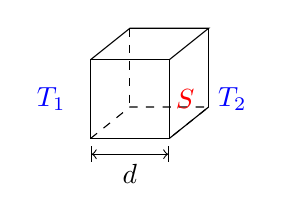
\begin{tikzpicture}
    % Box
    \draw (0,0) -- ++(1,0) -- ++(0,1) -- ++(-1,0) -- cycle;
    \draw[dashed] (0,0) -- ++(0.5,0.4) -- ++(1,0) -- ++(-0.5,-0.4);
    \draw (0,1) -- ++(0.5,0.4) -- ++(1,0) -- ++(-0.5,-0.4);
    \draw[dashed] (0.5,1.4) -- ++(0,-1);
    \draw (1.5,1.4) -- ++(0,-1);
    \draw (1,0) -- ++(0.5,0.4);
    
    \node[red] at (1.2,0.5){$S$};
    \node[blue] at (-0.5,0.5){$T_1$};
    \node[blue] at (1.8,0.5){$T_2$};
    \draw[|<->|] (0,-0.2) -- ++(1,0)
      node[pos=0.5,below]{$d$};
  \end{tikzpicture}
\end{center}
Se un corpo presenta una differenza di temperatura tra le sue pareti ci sarà uno scambio di calore
$Q$
\begin{equation*}
  \frac{Q}{\Delta t} = \frac{\mu S}{d\Delta T}
\end{equation*}
$\mu$: conducibilità termica\\
$S$: superficie\\
$d$: spessore del corpo\\
$\Delta T$: variazione di temperatura

\subsubsection{Temperatura di equilibrio}
Due sistemi sono in equilibrio termico quando hanno la stessa temperatura\\
La temperatura di equilibrio è la temperatura finale che raggiungono due sistemi a contatto fra di 
loro. Quando non sono in equilibrio, ci sarà uno scambio di calore.
\begin{equation*}
  t_e = \frac{m_1c_1t_1 + m_2c_2t_2}{m_1c_2 + m_2c_2}
\end{equation*}
$_1$: relativo al primo corpo\\
$_2$: relativo al secondo corpo

\subsubsection{Calore latente}
Il calore latente è la quantità di calore scambiata nel passaggio di fase di un corpo. Ogni 
passaggio necessita di energia diversa e quindi di coefficienti diversi.
\begin{equation*}
  Q_L = c_Lm
\end{equation*}
$c_L$: calore latente, diverso dal \emph{calore specifico}

\subsubsection{Passaggi di stato}
\begin{center}
  \begin{tikzpicture}
    \coordinate (O) at (0,0);
    \coordinate (O1) at (0,2.5);
    \coordinate (O2) at (6.5,0);

    \coordinate (A) at (0.75,1);
    \coordinate (B) at (2,1);
    \coordinate (C) at (3.5,1.75);
    \coordinate (D) at (5,1.75);
    \coordinate (E) at (6, 2);

    \draw[-stealth] (O) -- (O1)
      node[pos=1, left]{$T$};
    \draw[-stealth] (O) -- (O2)
      node[pos=1, below]{$Q_L$};

    \filldraw[olive, fill opacity = 0.3] (O) -- (A) -- (A |- O);
    \filldraw[green, fill opacity = 0.3] (A |- O) -- (A) -- (B) -- (B |- O);
    \filldraw[blue, fill opacity = 0.3] (B |- O) -- (B) -- (C) -- (C |- O);
    \filldraw[cyan, fill opacity = 0.3] (C |- O) -- (C) -- (D) -- (D |- O);

    \draw (O) -- (A) -- (B) -- (C) -- (D) -- (E);

    \draw[dashed] (A -| O) -- (A)
      node[pos=0, left]{$T_f$};
    \draw[dashed] (C -| O) -- (C)
      node[pos=0, left]{$T_v$};

    \node[rotate=60, below] at ($(O)!0.5!(A)$) {Solido};
    \node[text width=1.5cm, anchor=south, xshift=0.3cm, yshift=-1cm] at ($(A)!0.5!(B)$) 
      {Solido e liquido};
    \node[text width=1.5cm, anchor=south, xshift=0.3cm, yshift=-1cm] at ($(B)!0.5!(C)$) 
      {Liquido};
    \node[text width=1.5cm, anchor=south, xshift=0.2cm, yshift=-1.3cm] at ($(C)!0.5!(D)$) 
      {Liquido e vapore};
    \node[text width=1.5cm, anchor=south, xshift=0.5cm, yshift=-1.4cm] at ($(D)!0.5!(E)$) 
      {Vapore};
    \node[text width=1.5cm, anchor=south, xshift=0.3, yshift=-1.6cm] at ($(A)!0.5!(B)$)
      {$Q_f=\lambda_f\cdot m$};
    \node[text width=1.5cm, anchor=south, xshift=0.3, yshift=-2.3cm] at ($(C)!0.5!(D)$)
      {$Q_v=\lambda_v\cdot m$};
    \draw (2.1,1.9) to[bend left] ($(B)!0.5!(C)$);
    \node at (1.3,2.3){$c=\frac{Q}{m\cdot\Delta T}$};
  \end{tikzpicture}
\end{center}
Questo grafico rappresenta indicantivamente i passaggi di stato. Si può leggere sia da sinistra che da 
destra, ovvero che dal grafico si può capire che in modulo, l'energia necessaria per fare solidificare
il corpo, è pari a quella necessaria per farlo liquefare.

\subsubsection{Conversione da J a cal}
Essendo entrambi unità di misura dell'energia, è possibile convertire una dall'altra.
\begin{equation*}
  1\,\text{cal} = 4.184\,\text{J}
\end{equation*}


\subsection{Termodinamica (Lavoro)}
\begin{equation*}
  Q = L+\Delta U
\end{equation*}
$Q$: quantità di calore\\
$L$: lavoro\\
$\Delta U$: variazione di energia interna

\subsubsection{Tabella per i segni di $Q$ e $L$}
La seguente tabella riassume in breve i segni che la quantità di calore e il lavoro devono avere.
\tablefirsthead{\toprule Segno &  $Q$ & $L$ \\ \midrule}
\tablehead{Segno & $Q$ & $L$ \\ \midrule}
\tablelasttail{\bottomrule}
\begin{center}
  \begin{xtabular}{M{2cm} M{2cm} M{2cm}}
    Positivo & Il sistema acquista energia dall'esterno mediante uno scambio di calore &
    Il sistema compie un lavoro positivo (durante un'espansione) e cede energia\\ \midrule
    Negativo & Il sistema cede energia all'esterno mediante uno scambio di calore &
    Il sistema compie un lavoro negativo (durante una compressione) e acquista energia\\
  \end{xtabular}
\end{center}
\subsubsection{Trasformazione isobara}
Un'isobara è una trasforamazione che mantiene costante la pressione.
\begin{equation*}
  L = p\Delta V
\end{equation*}
\begin{equation*}
  Q = c_pnR\Delta T=\frac{2+l}{2}nR\Delta T
\end{equation*}
\begin{equation*}
  \Delta U = \frac{l}{2}nR\Delta T
\end{equation*}
\hyperref[tab:R]{$R$}: $0.0821\,\text{l}\cdot\text{atm/n}\cdot\text{K}$
$8.31\,\text{J/K}\cdot\text{mol}$\\
$c_p$: è il calore specifico di un corpo sottoposto a una trasformazione isobara

\subsubsection{Trasformazione isoterma}
Un'isoterma è una trasformazione che mantiene costante la temperatura.
\begin{align*}
  \Delta U &= 0\\
  L &= Q = nRT\ln\frac{V_2}{V_1}
\end{align*}
\hyperref[tab:R]{$R$}: $0.0821\,\text{l}\cdot\text{atm/n}\cdot\text{K}$
$8.31\,\text{J/K}\cdot\text{mol}$\\

\subsubsection{Trasformazione isocora}
Un'isocora è una trasformazione che mantiene costante il volume.
\begin{equation*}
  L = 0
\end{equation*}
\begin{equation*}
  Q = \Delta U = c_VnR\Delta T =\frac{l}{2}nR\Delta T
\end{equation*}
\hyperref[tab:R]{$R$}: $0.0821\,\text{l}\cdot\text{atm/n}\cdot\text{K}$
$8.31\,\text{J/K}\cdot\text{mol}$\\
$c_V$: è il calore specifico di un corpo sottoposto a una trasformazione isocora

\subsubsection{Lavoro di un ciclo}
\begin{center}
  \begin{tikzpicture}[scale=0.75]
    \coordinate (A) at (1,2);
    \coordinate (B) at (2,2);
    \coordinate (C) at (2,4);
    \coordinate (D) at (3.5,2.5);
    \coordinate (E) at (4.5,1);
    \coordinate (F) at (1,1);

    \draw[-stealth] (-0.5,0) -- (5,0)
      node[pos=1, below]{$V$};
    \draw[-stealth] (0,-0.5) -- (0,5)
      node[pos=1,left]{$p$};
    \path[thick, -stealth] 
      (A) edge (B) 
      (B) edge (C) 
      (C) edge[bend right=20] (D) 
      (D) edge[bend right=30] (E)
      (E) edge (F)
      (F) edge (A);

    \node[anchor=south, yshift=-0.6cm, xshift=0.6cm] at ($(A)!0.5!(B)$){Isobara};
    \node[anchor=south, yshift=-0cm, xshift=-0.6cm] at ($(B)!0.5!(C)$){Isocora};
    \node[above right] at ($(C)!0.5!(D)$){Isoterma};
    \node[right] at ($(D)!0.5!(E)$){Adiabatica};

    \draw[decorate, decoration={snake}, red, ->] (1.5,2.5) -- ++(0.9,0);
    \draw[decorate, decoration={snake}, red, ->] (1.5,2.2) -- ++(0,-0.7);
    \draw[decorate, decoration={snake}, red, ->] (3,3.3) -- ++(-0.5,-0.5);
    \draw[decorate, decoration={snake}, red, ->] (0.5,1.5) -- ++(0.9,0);
    \draw[decorate, decoration={snake}, blue, ->] (3.3,1.5) -- ++(0,-0.9);
  \end{tikzpicture}
\end{center}
In rosso è se $Q > 0$, in blu se $Q<0$.
\begin{equation*}
  L = \sum\limits_{i=0}^{n} Q_i
\end{equation*}
Il lavoro è anche pari all'area occpuata dal ciclo (N/$\text{m}^2\text{m}^3$).\\
Si noti anche che in generale se il ciclo ``va'' in senso orario, il lavoro sarà positivo,
negativo altrimenti.

\subsubsection{Trasformazione adiabatica}
Un'adiabatica è una trasformazione che non cede calore all'esterno quindi $Q=0$ e
\begin{equation*}
  L = -\Delta U
\end{equation*}
Queste seguenti, sono definite \textbf{Equazioni di Poisson}
\begin{equation*}
  pV^\gamma = \text{costante}
\end{equation*}
\begin{equation*}
  V_1^{\gamma-1}T_1 = V_2^{\gamma-1}T_2
\end{equation*}
\begin{equation*}
  p_1^{1-\gamma}T_1^\gamma = p_2^{1-\gamma}T_2^\gamma
\end{equation*}
$\gamma$: rapporto tra $c_p$ e $c_V$\\ [\baselineskip] 
La seguente tabella riassume i valori di $\gamma$ e calore specifico a pressione e volume costante:
\begin{center}
  \begin{tabular}{c | c | c | c}
    Tipo di gas & $c_p$ & $c_V$ & $\gamma=\frac{c_p}{c_V}$\\ \hline
    Monoatomico & $\frac{5}{2}R$ & $\frac{3}{2}R$ & $1.\bar{6}$\\ \hline
    Biatomico & $\frac{7}{2}R$ & $\frac{5}{2}R$ & $1.4$\\
  \end{tabular}
\end{center}


\subsubsection{Macchina di Carnot}
Una macchina termica è un dispositivo che efettua trasformazioni cicliche (ad esempio un motore
di un'automobile).\\
La macchina di Carnot è la più efficiente di tutte che lavora tra le temperature $T_1$ e $T_2$.
\begin{center}
  \begin{tikzpicture}
    \filldraw[orange, fill opacity=0.3] (0,0) -- (0,0.5) -- (2,0.5) -- (2,0);
    \filldraw[cyan, fill opacity=0.3] (0,2.5) -- (0,2) -- (2,2) -- (2,2.5);

    \filldraw[gray, fill opacity=0.3] (1,1.25) circle (0.5);

    \draw[line width=0.5mm,-implies,double, double distance=1mm] (1,0.4) -- (1,1.15)
      node[pos=0.4, anchor=east, xshift=-.2cm]{$Q_2$};
    \draw[line width=0.5mm,-implies,double, double distance=1mm] (1,1.5) -- (1,2.15)
      node[pos=0.4, anchor=east, xshift=-.2cm]{$Q_1$};
    \draw[line width=0.5mm,-implies,double, double distance=1mm] (1.5,1.25) -- (2,1.25)
      node[pos=0.4, anchor=east, xshift=1.5cm]{$L < Q_2$};
  \end{tikzpicture}
\end{center}
\begin{equation*}
  \eta = 1-\frac{\abs{Q_1}}{\abs{Q_2}} = \abs{\frac{L}{Q_2}}
\end{equation*}
\begin{equation*}
  \eta_c = 1 - \frac{T_1}{T_2}
\end{equation*}
$T_1$: sorgente fredda\\
$T_2$: sorgente calda\\ [\baselineskip]
La prima formula definisce il rendimento ($\eta$) di una qualsiasi macchina termica, la seconda solo
per una macchina di Carnot. $Q_1$ è il calore ceduto dalla sorgente fredda, $Q_2$ è quello fornito 
dalla sorgente calda\\
La macchina di Carnot dimostra che non può esserci una macchina con efficienza $1$ in quanto non
si può avere $T_1 = 0\,\text{K}$.\\ [\baselineskip]
La potenza in una macchina di Carnot è
\begin{equation*}
  P = \frac{Q_2\eta}{t} 
\end{equation*}
$P$: potenza\\
$\eta$: rendimento

\subsection{Entropia}\label{subsec:termodinamica:entropia}
Per definire l'entropia, definiamo la \textbf{disuguaglianza di Clausius} che ci aiuterà a capire la 
definizione di entropia.
\begin{equation*}
  \sum\limits_{i = 1}^{n}\frac{\Delta Q_i}{T_i} \leq 0
\end{equation*}
se il ciclo è reversibile si ha questa forma
\begin{equation*}
  \left(\sum\limits_{i = 1}^{n}\frac{\Delta Q_i}{T_i}\right)_\text{rev} = 0
\end{equation*}
L'\textbf{entropia} è in definitiva una formulazione più generale del secondo principio della 
termodinamica che sia appropriato per ogni trasformazione. L'entropia è una funzione di stato.\\
Per uno stato $C$ e uno stato di riferimento $R$ per cui $S(R) = 0\,\text{J/K}$, l'entropia è così 
definita:
\begin{equation*}
  S(C) = S(C) - S(R) = \left(\sum\limits_{i = 1}^{n}\frac{\Delta Q_i}{T_i}\right)_{\substack{R\to C\\
  \text{rev}}}
\end{equation*}
Per gli esercizi, si vada a pagina~\pageref{ex:entropia}.

\subsubsection{Proprietà dell'entropia}
L'entropia è una grandezza estensiva, ovvero che preso un sistema $\Omega$ che sia l'unione di due
sottositemi indipendenti $\Omega_1$ e $\Omega_2$ ($\Omega = \Omega_1 \cup \Omega_2$), la sua entropia
è pari a
\begin{align*}
  S(C) = \left(\sum\limits_{i=1}^{n}\frac{\Delta Q_i}{T_i}\right)_{\substack{R\to C\\\text{rev}}} &=\\ 
  \left(\sum\limits_{i=1}^{n}\frac{\Delta Q_i}{T_i}\right)^{\Omega_1}_{\substack{R\to C\\\text{rev}}} &+
  \left(\sum\limits_{i=1}^{n}\frac{\Delta Q_i}{T_i}\right)^{\Omega_2}_{\substack{R\to C\\\text{rev}}}
\end{align*}

\subsubsection{Entropia di un sistema isolato}
In un sistema isolato l'entropia ha una variazione pari a \textbf{zero} solo se la trasformazione è
\textit{reversibile}, \textbf{maggiore di zero} altrimenti.

\subsubsection{Entropia dell'universo}
L'entropia dell'universo è sempre in crescita in quanto avvengono trasformazioni irreversibili senza
fine (come ad esempio un'esplosione).

\subsubsection{Entropia di un sistema non isolato}
Se una trasformazione reale provoca in un un sistema una diminuzione di entropia pari a 
$\vert \Delta S \vert$, nel resto dell'universo è maggiore di $\vert \Delta S \vert$.

\subsubsection{Macrostati e microstati}
Un \emph{microstato} è una precisa combinazione di elementi microscopici, un \emph{macrostato} è 
descritto dalle variabili macroscopiche che ne descrivono le proprietà.\\
Ad esempio: un macrostato per un sistema termodinamico è descritto da almeno due delle tipiche 
variabili (pressione, volume e temperatura). Un microstato invece è lo stato di ogni molecola di gas 
nel sistema.\\
Un microstato corrisponde ad un solo macrostato, un macrostato può essere descritto da più macrostati.
Si noti anche che più un macrostato è disordinato, più è probabile che si realizzi spontaneamente.

\subsubsection{Molteplicità di un macrostato}
Sia $A$ un macrostato. Si definisce $W(A)$ come \textbf{molteplicità}, ovvero il numero di microstati 
distinti che corrispondono ad $A$.

\begin{center}
  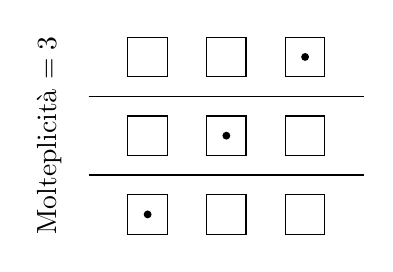
\begin{tikzpicture}
    \draw (0,0) -- ++(0.5,0) -- ++(0,-0.5) -- ++(-0.5,0) -- cycle;
    \draw (1,0) -- ++(0.5,0) -- ++(0,-0.5) -- ++(-0.5,0) -- cycle;
    \draw (2,0) -- ++(0.5,0) -- ++(0,-0.5) -- ++(-0.5,0) -- cycle;
    \fill (0.25,-0.25) circle(0.05);

    \draw (-0.5,1.25) -- ++(3.5,0);

    \draw (0,1) -- ++(0.5,0) -- ++(0,-0.5) -- ++(-0.5,0) -- cycle;
    \draw (1,1) -- ++(0.5,0) -- ++(0,-0.5) -- ++(-0.5,0) -- cycle;
    \draw (2,1) -- ++(0.5,0) -- ++(0,-0.5) -- ++(-0.5,0) -- cycle;
    \fill (1.25,0.75) circle(0.05);

    \draw (-0.5,0.25) -- ++(3.5,0);

    \draw (0,2) -- ++(0.5,0) -- ++(0,-0.5) -- ++(-0.5,0) -- cycle;
    \draw (1,2) -- ++(0.5,0) -- ++(0,-0.5) -- ++(-0.5,0) -- cycle;
    \draw (2,2) -- ++(0.5,0) -- ++(0,-0.5) -- ++(-0.5,0) -- cycle;
    \fill (2.25,1.75) circle(0.05);

    \node at (-1,0.75){\rotatebox{90}{{Molteplicità $=3$}}};
  \end{tikzpicture}
\end{center}

\subsubsection{Equazione di Boltzman}
\begin{equation*}
  S(A) = k_B\ln W(A)
\end{equation*}
\hyperref[tab:kB]{$k_B$}: $1.318\cdot10^{-23}\,\text{J/K}$
